\documentclass[12pt,a4paper]{report}
\usepackage[utf8]{inputenc}
\usepackage{graphicx}
\usepackage{geometry}
\usepackage[hidelinks]{hyperref} % [hidelinks] removes the red boxes around the TOC items
\usepackage{listings}
\usepackage{xcolor}
\usepackage{float}
\usepackage{titlesec}
\usepackage{caption}

% Set page margins
\geometry{
    top=1in,
    bottom=1in,
    left=1in,
    right=1in
}

% Code snippet styling
\definecolor{codegreen}{rgb}{0,0.6,0}
\definecolor{codegray}{rgb}{0.5,0.5,0.5}
\definecolor{codepurple}{rgb}{0.58,0,0.82}
\definecolor{backcolour}{rgb}{0.95,0.95,0.92}

\lstdefinestyle{mystyle}{
    backgroundcolor=\color{backcolour},   
    commentstyle=\color{codegreen},
    keywordstyle=\color{magenta},
    numberstyle=\tiny\color{codegray},
    stringstyle=\color{codepurple},
    basicstyle=\ttfamily\footnotesize,
    breakatwhitespace=false,         
    breaklines=true,                 
    captionpos=b,                    
    keepspaces=true,                 
    numbers=left,                    
    numbersep=5pt,                  
    showspaces=false,                
    showstringspaces=false,
    showtabs=false,                  
    tabsize=2
}
\lstset{style=mystyle}

\begin{document}

% =======================================================
% 1. Title Page
% =======================================================
\begin{titlepage}
    \centering
    \vspace*{2cm}
    
    {\Huge \textbf{Campus Lost \& Found Portal}}\\[0.5cm]
    {\LARGE \textbf{Final Project Report}}\\[2cm]
    
    {\Large \textbf{Course:}} \\ Web Application Development\\[0.5cm]
    
    {\Large \textbf{Project ID:}} \\ 119577\\[1.5cm]
    
    {\Large \textbf{Project Members:}}\\[0.5cm]
    \begin{tabular}{ll}
        \textbf{Name} & \textbf{Student ID} \\
        \hline \\[-0.8em]
        Mohyuddiin & 65405 \\
        Zain Imran & 65495 \\
        Shahzaman Khan & 64930 \\
    \end{tabular}\\[3cm]
    
    {\large \textbf{Date:}} \\ \today
    
    \vfill
\end{titlepage}

\tableofcontents
\newpage

% =======================================================
% 2. Project Documentation
% =======================================================
\chapter{Project Documentation}

\section{Introduction}
The \textbf{Campus Lost \& Found Portal} is a web application designed to help students and staff report lost items and browse found items posted by others. It solves a common everyday problem on any campus or institution where items get misplaced and there is no organized way to reunite them with their owners. 

\section{Problem Statement}
When someone loses an item on campus, they have no easy way to check if it has been found and handed in somewhere. Similarly, someone who finds an item has no reliable way to reach its owner. Currently, people rely on notice boards or word of mouth, which is slow and ineffective. This portal provides a centralized, searchable solution to this problem.

\section{Objectives}
\begin{itemize}
    \item Allow users to register and log in to the portal securely.
    \item Let users post a lost item or a found item with details and an optional photo.
    \item Allow anyone to browse and search posted items by category or location.
    \item Let a user mark an item as returned/resolved once it is claimed.
    \item Build the application using ASP.NET MVC, C\#, HTML, and CSS.
\end{itemize}

\section{Key Features}
\begin{itemize}
    \item \textbf{User Registration \& Login:} Secure accounts using ASP.NET Identity.
    \item \textbf{Post Lost Item:} Title, description, date lost, location, category (e.g. bag, phone, keys), and image upload capabilities.
    \item \textbf{Post Found Item:} Same fields but from the finder's perspective.
    \item \textbf{Browse \& Search:} View all active posts, filter by category or location keyword.
    \item \textbf{Mark as Resolved:} The post owner can close a listing once the item is returned.
    \item \textbf{My Posts:} A personal dashboard page showing only the logged-in user's listings.
\end{itemize}

\section{System Architecture}
The application strictly adheres to the \textbf{Model-View-Controller (MVC)} architectural pattern:
\begin{itemize}
    \item \textbf{Models:} Defines the core data structures (Item, ApplicationUser, Claim, Notification, Building, Category). Relationships are managed via Entity Framework (EF) Core Fluent API and Data Annotations.
    \item \textbf{Controllers:} Handles business logic and HTTP requests (ItemsController, AdminController, NotificationsController, ProfileController).
    \item \textbf{Views:} Razor Pages (.cshtml) strongly typed to ViewModels, utilizing a shared Layout for a consistent UI.
\end{itemize}

\section{Technology Stack}
\begin{table}[H]
\centering
\begin{tabular}{|l|l|}
\hline
\textbf{Layer} & \textbf{Technology} \\ \hline
Front-End & HTML5, CSS3, Razor Views (.cshtml), Bootstrap 5 \\ \hline
Back-End & ASP.NET Core MVC, C\# \\ \hline
Database & Microsoft SQL Server, Entity Framework Core (Code-First) \\ \hline
Auth & ASP.NET Core Identity \\ \hline
IDE & Visual Studio 2022 \\ \hline
\end{tabular}
\end{table}

\section{Project Timeline}
\begin{table}[H]
\centering
\begin{tabular}{|c|l|}
\hline
\textbf{Week} & \textbf{Task} \\ \hline
1 & Project setup, database design, Git repository \\ \hline
2 & User registration and login (ASP.NET Identity) \\ \hline
3 & Lost \& Found item model and CRUD operations \\ \hline
4 & Browse, search, and filter functionality \\ \hline
5 & Image upload and My Posts page \\ \hline
6 & Mark as resolved feature and UI styling \\ \hline
7 & Testing and bug fixes \\ \hline
8 & Final review and submission \\ \hline
\end{tabular}
\end{table}

\section{Work Distribution}
\begin{table}[H]
\centering
\begin{tabular}{|p{3cm}|p{2cm}|p{8cm}|}
\hline
\textbf{Name} & \textbf{ID} & \textbf{Responsibility} \\ \hline
Mohyuddiin & 65405 & Back-end: Controllers, routing, ASP.NET Identity, C\# logic \\ \hline
Zain Imran & 65495 & Database: EF models, migrations, CRUD operations \\ \hline
Shahzaman Khan & 64930 & Front-end: HTML/CSS views, Razor templates, UI design \\ \hline
\end{tabular}
\end{table}

\section{Conclusion}
The Campus Lost \& Found Portal is a practical and unique web application that addresses a real problem students face every day. It is straightforward enough to build within the course timeframe while covering all required technologies: HTML, CSS, ASP.NET MVC, and C\#. The project involves user authentication, database interaction, image handling, and a clean searchable interface, making it a well-rounded and successfully implemented course project.

% =======================================================
% 3. Screen Shots
% =======================================================
\chapter{System Screenshots}

\section{Home Page (Dashboard)}
The main dashboard featuring a modern dark-mode design and quick stats.
\begin{figure}[H]
    \centering
    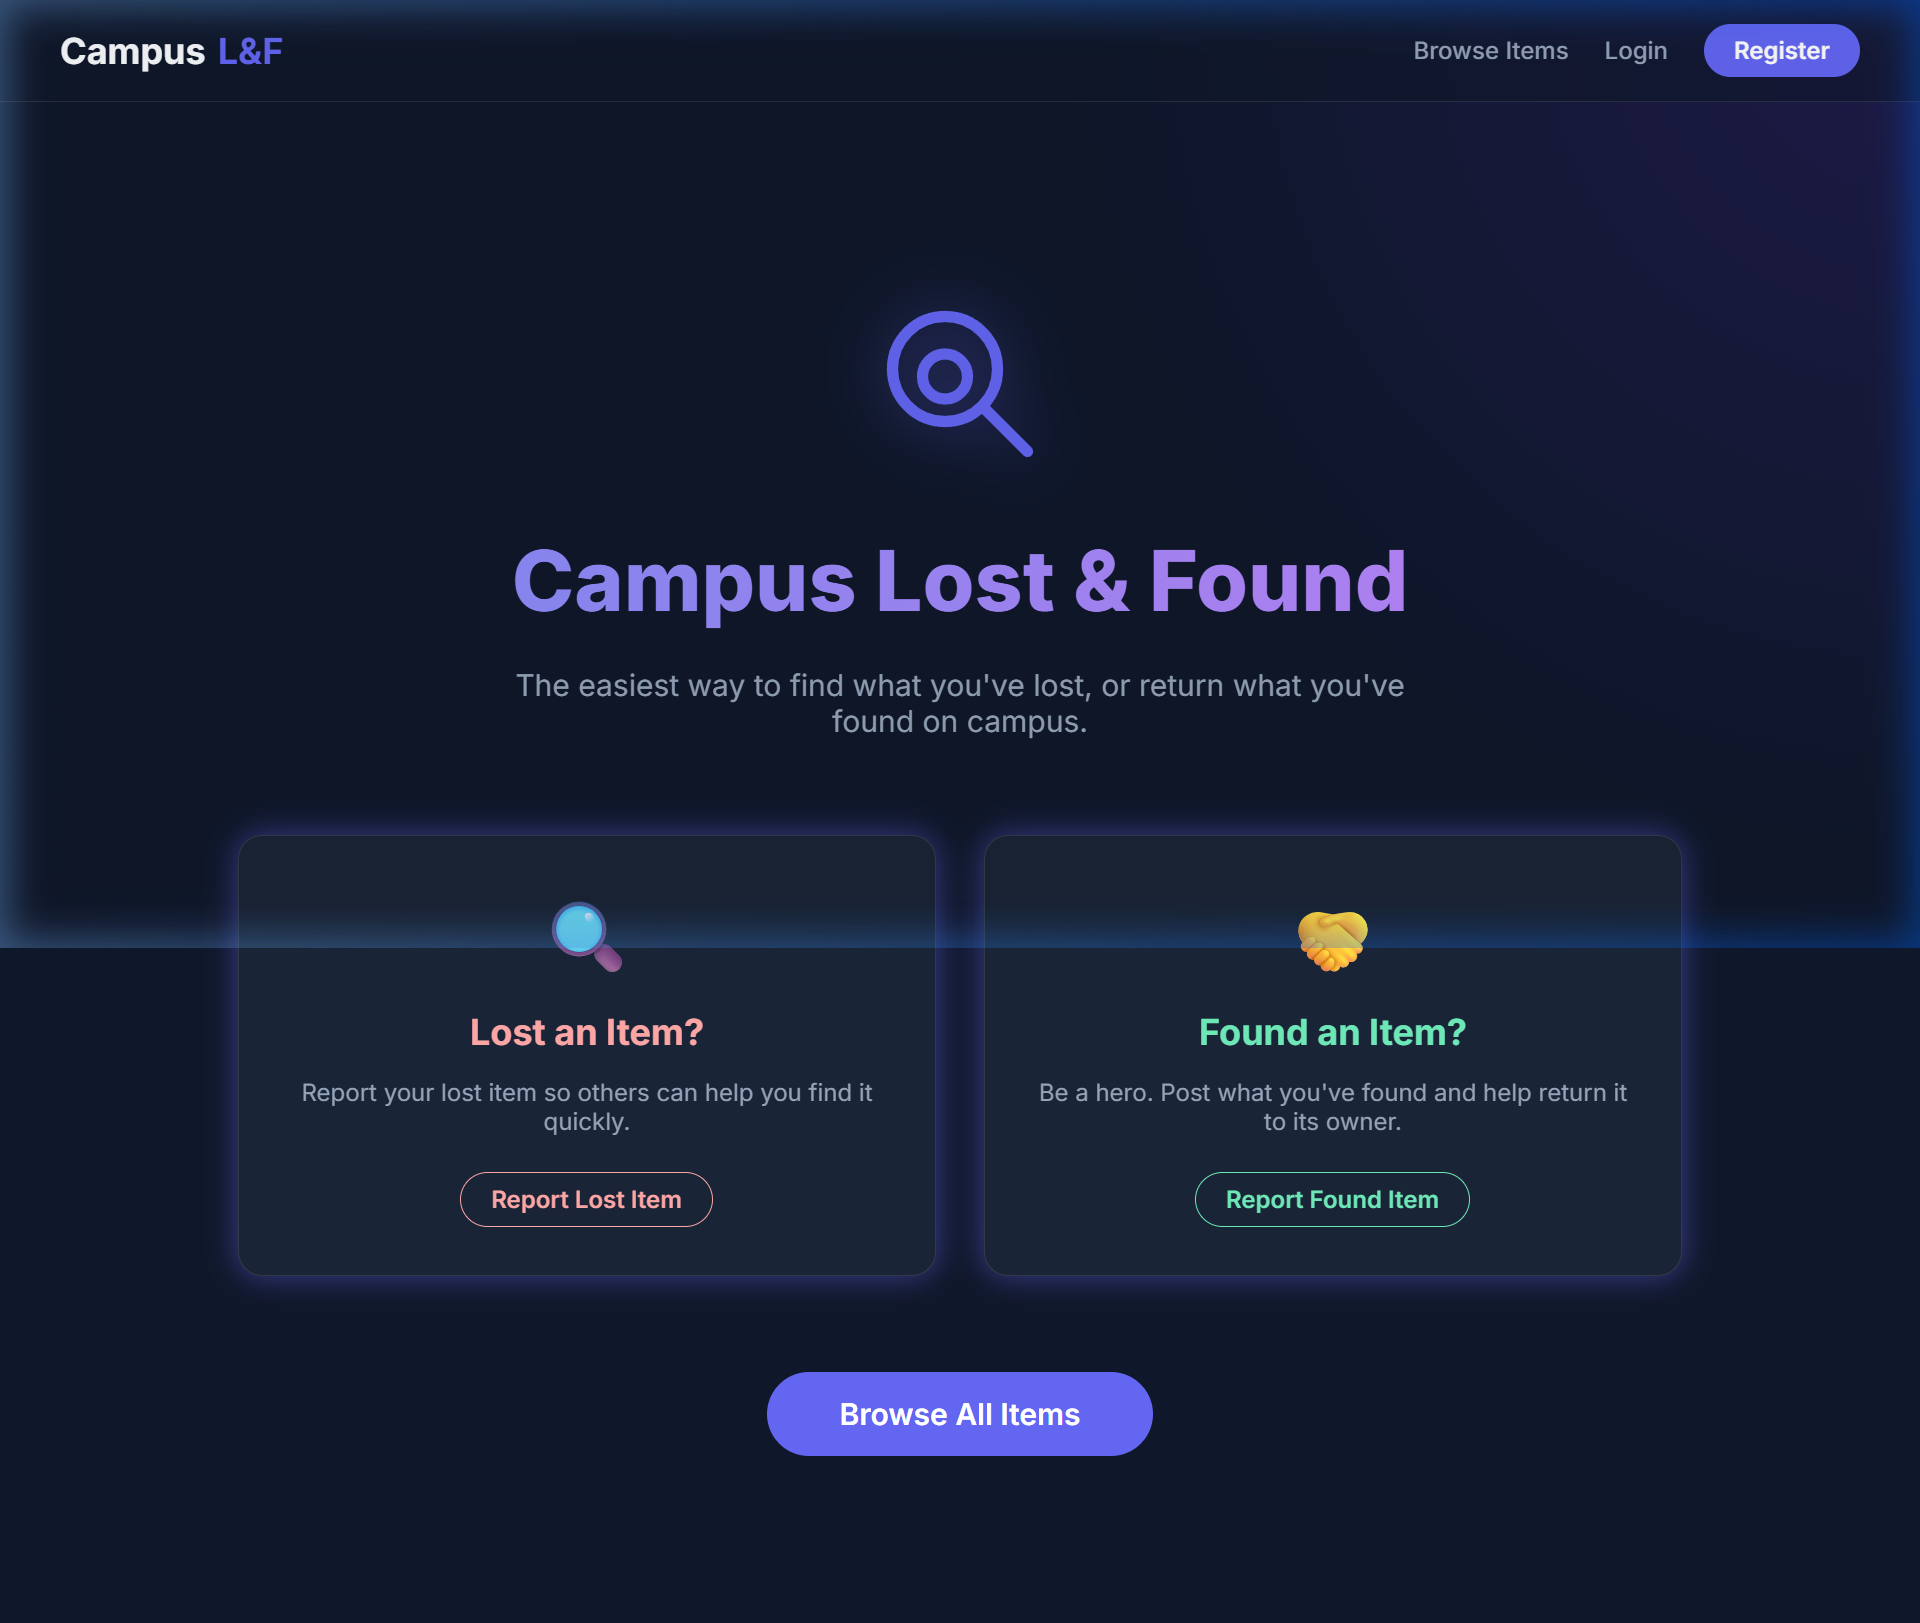
\includegraphics[width=0.9\textwidth]{1_Home_Page.png}
    \caption{Home Page Interface}
\end{figure}

\section{User Authentication (Login)}
A secure login portal utilizing ASP.NET Core Identity.
\begin{figure}[H]
    \centering
    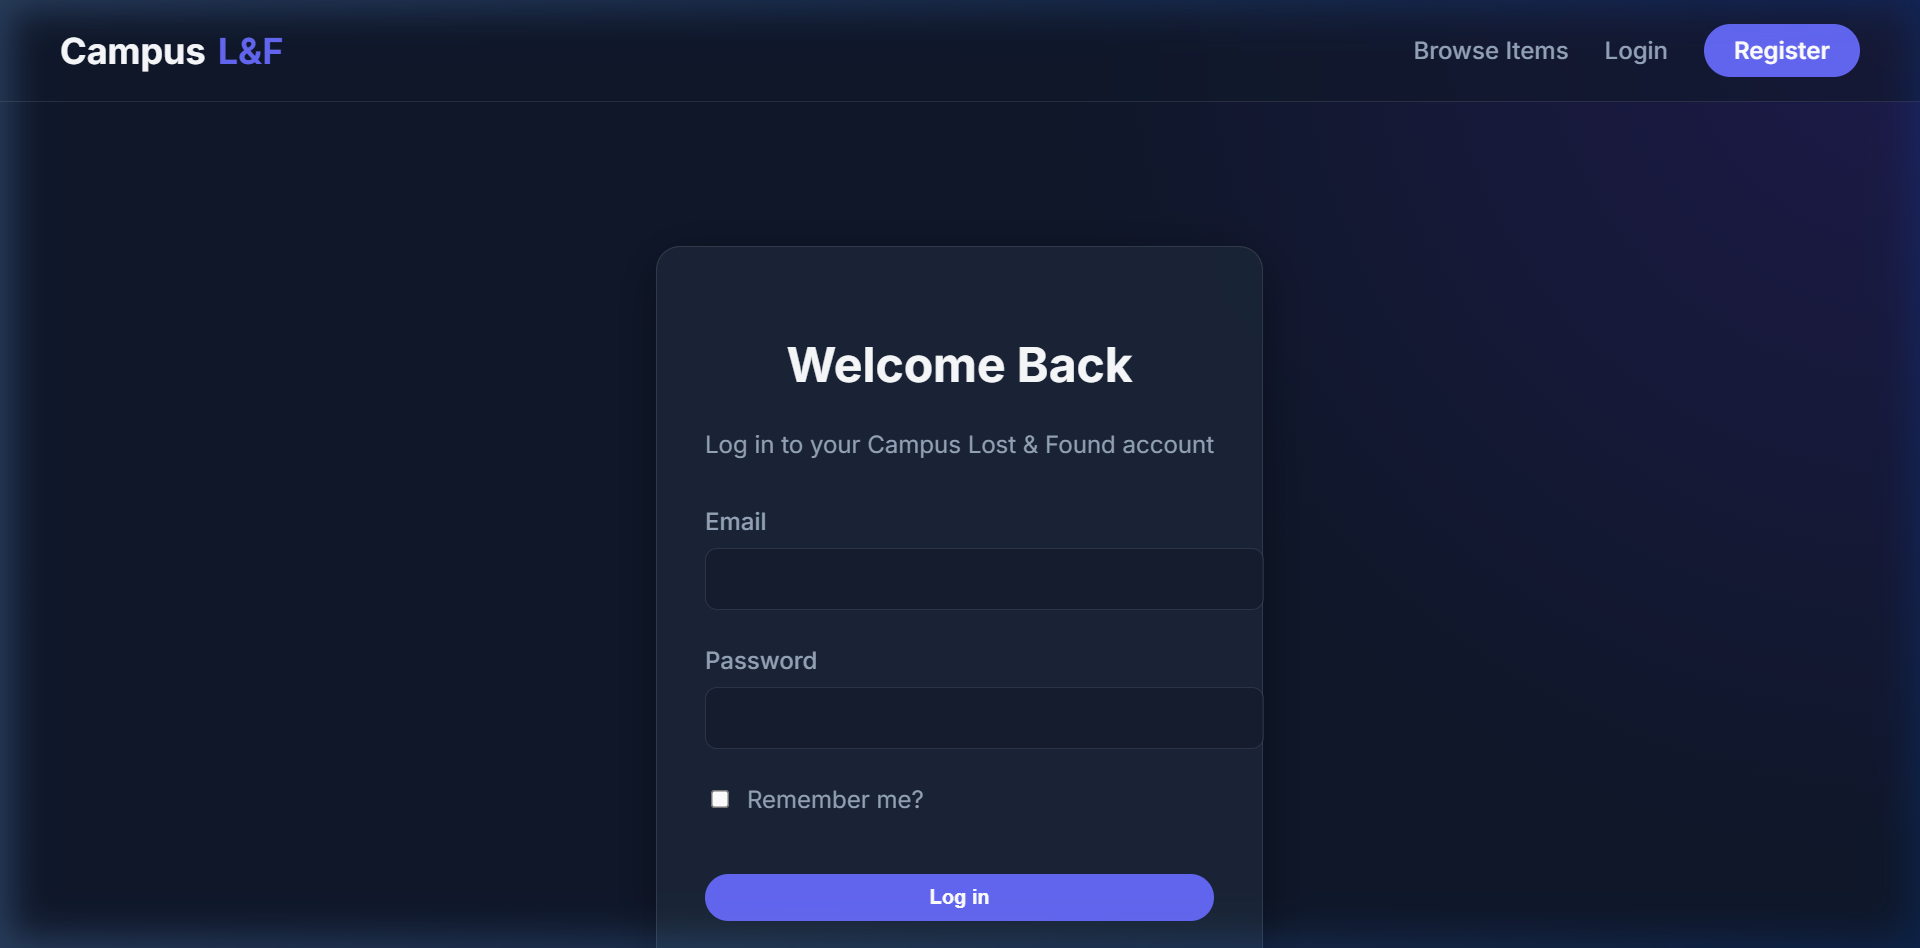
\includegraphics[width=0.9\textwidth]{2_Login_Page.png}
    \caption{Login Page}
\end{figure}

\section{Post an Item}
A secure and categorized form allowing users to post lost or found items.
\begin{figure}[H]
    \centering
    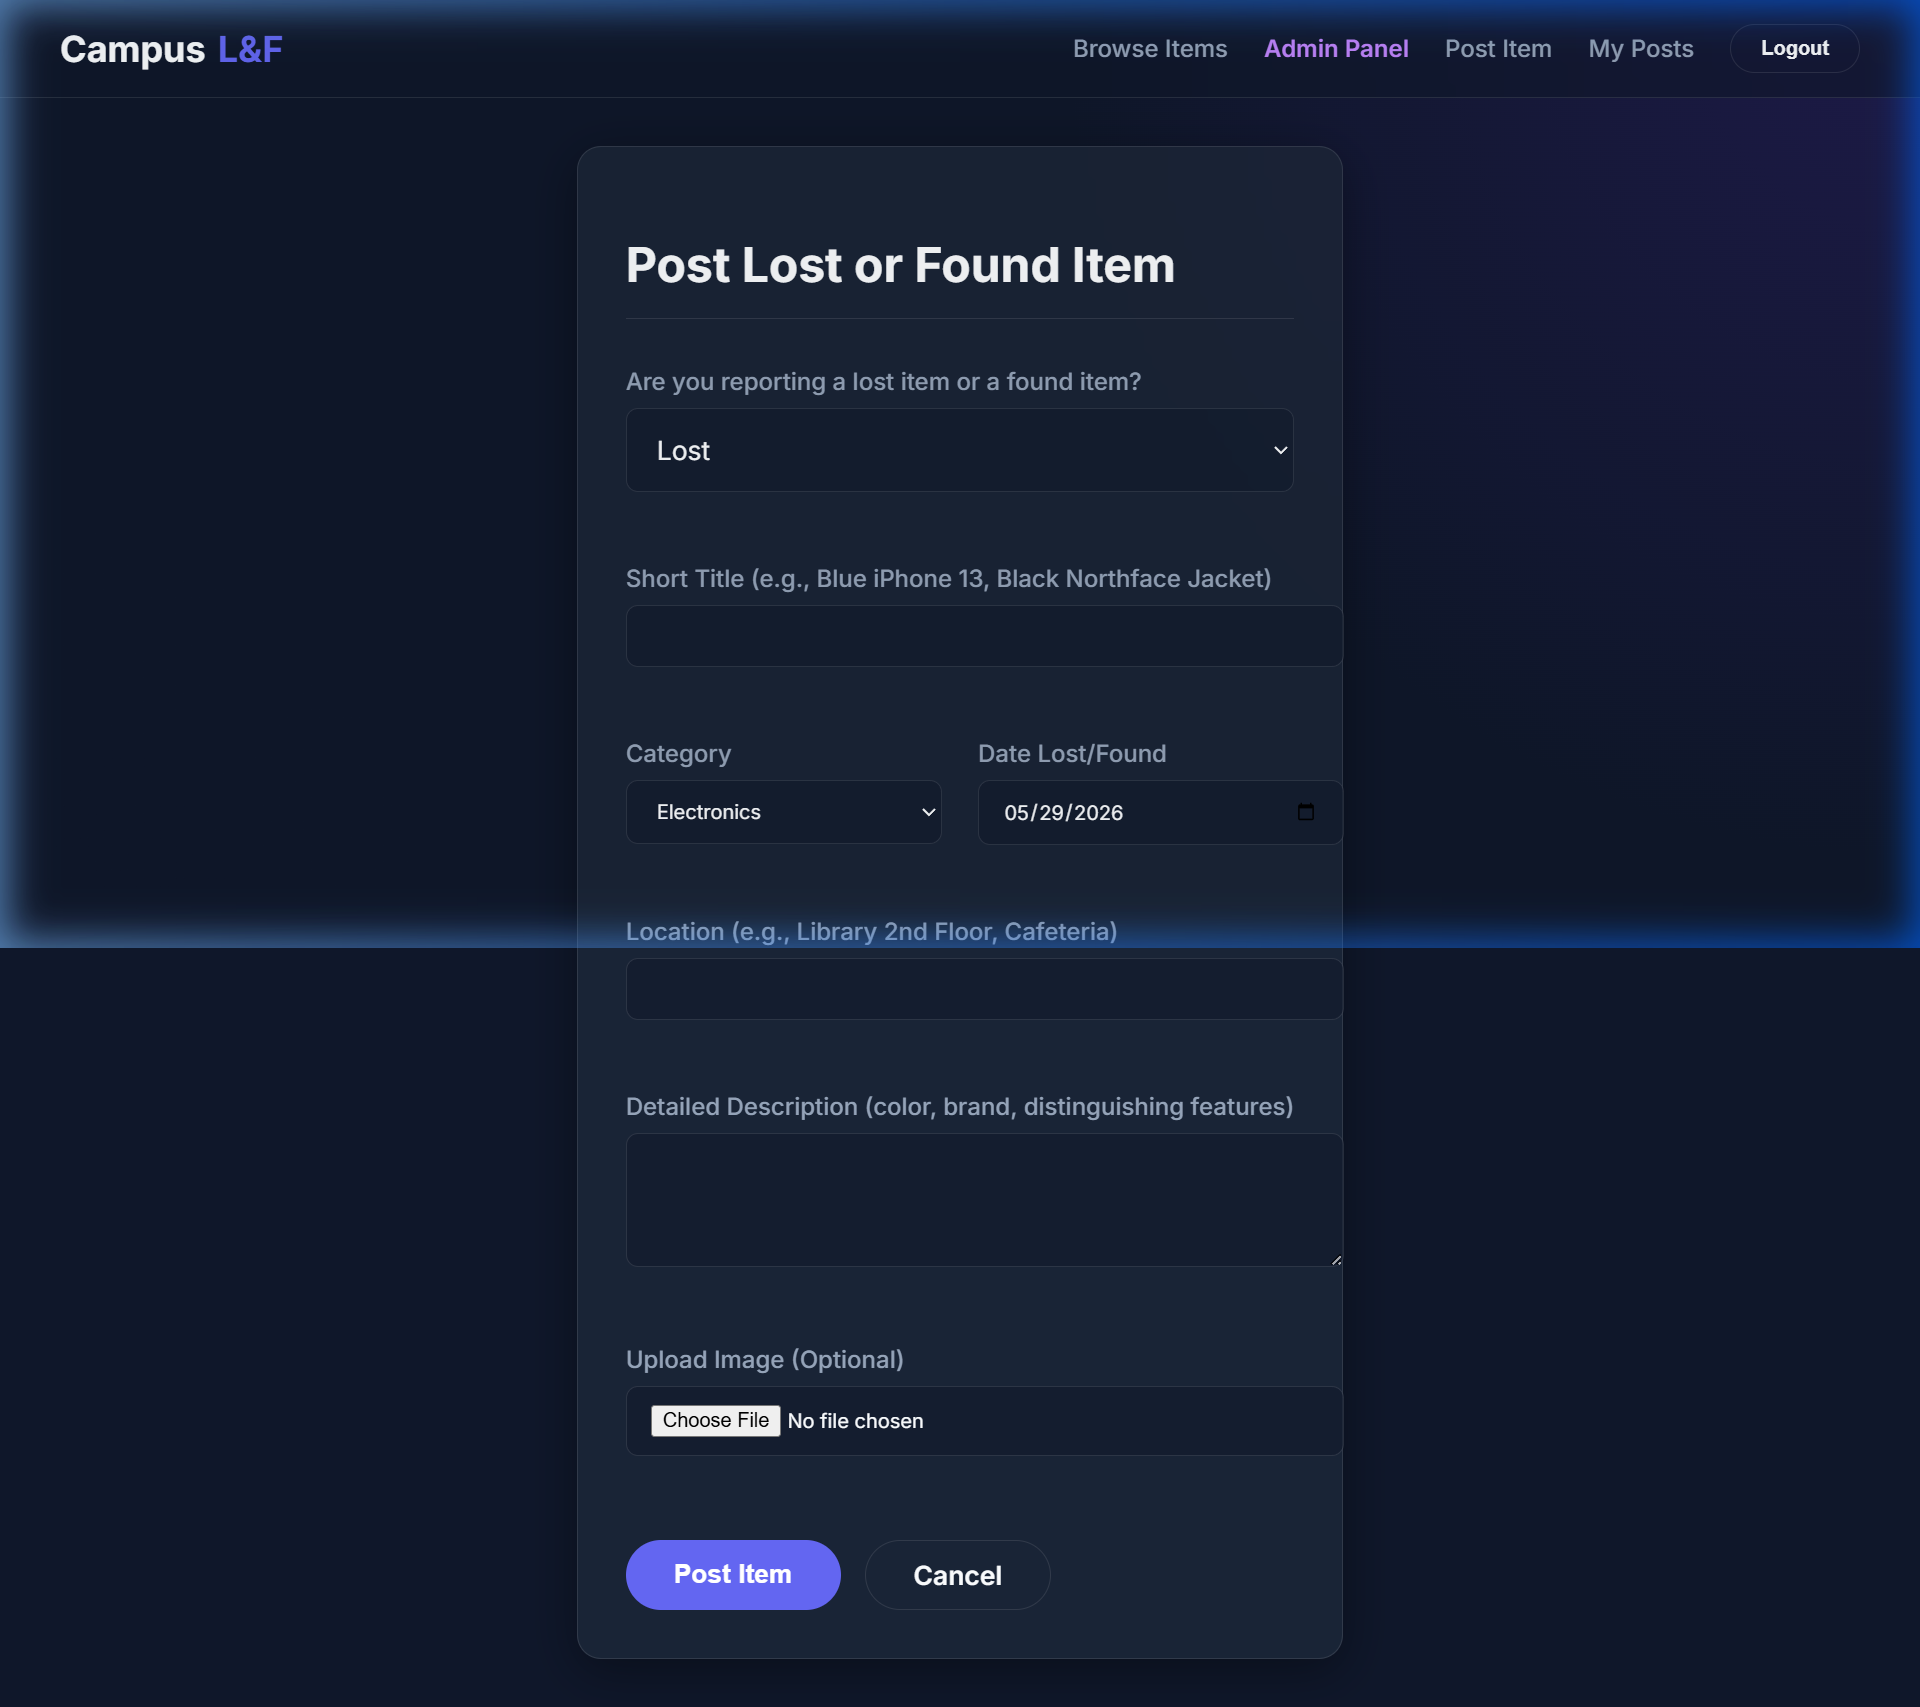
\includegraphics[width=0.9\textwidth]{3_Post_Item.png}
    \caption{Post Item Form}
\end{figure}

\section{Browse Items}
An organized grid displaying active items across the campus.
\begin{figure}[H]
    \centering
    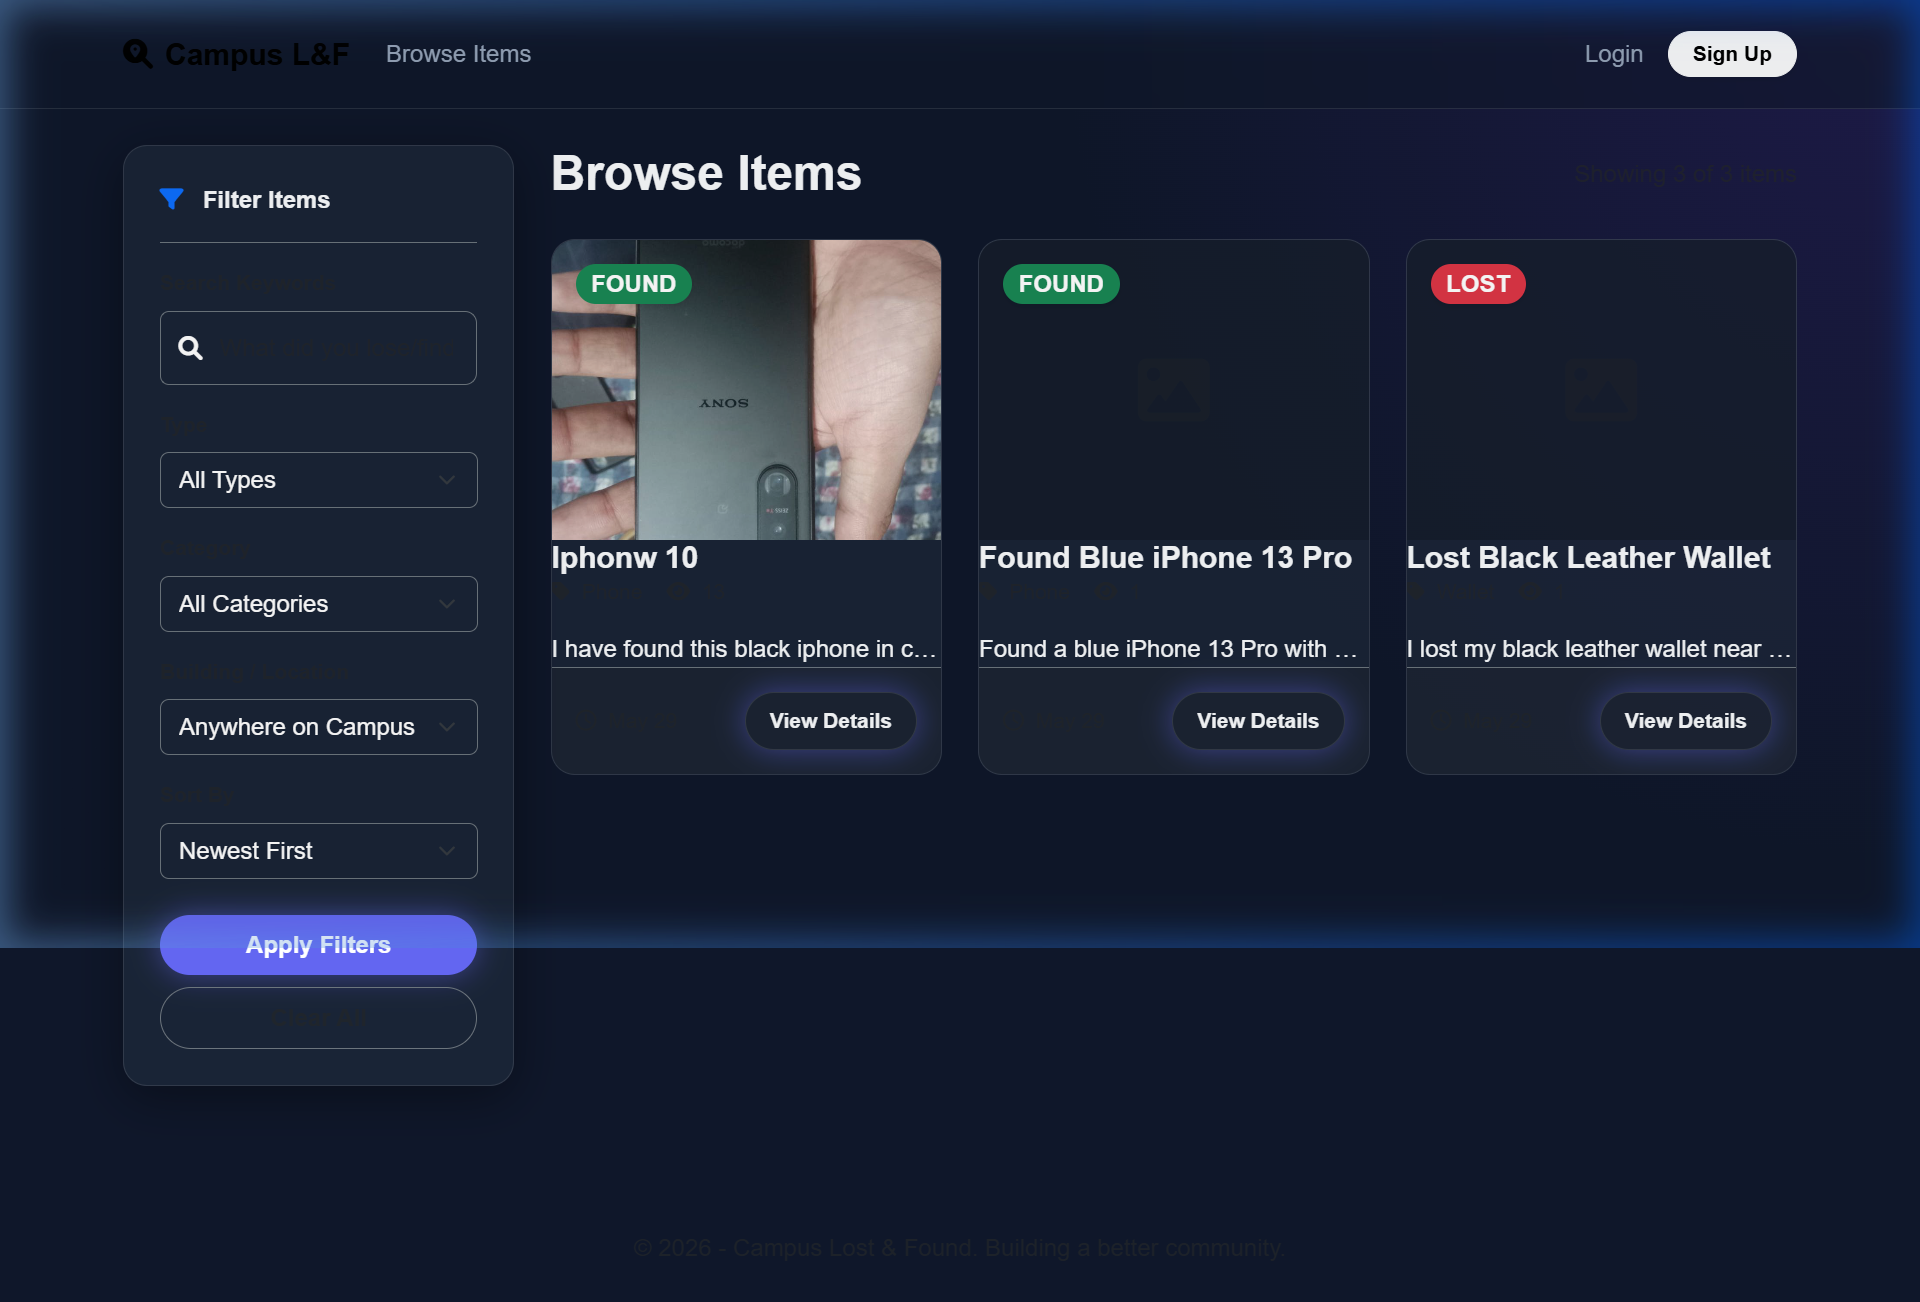
\includegraphics[width=0.9\textwidth]{4_Browse_Items.png}
    \caption{Item Browsing Interface}
\end{figure}

% =======================================================
% 4. Coding
% =======================================================
\chapter{Core Source Code}

Below is the detailed core source code demonstrating the system architecture and background processing jobs.

\section{Program.cs - Application Startup \& Configuration}
\begin{lstlisting}[language={[Sharp]C}]
using Hangfire;
using Microsoft.AspNetCore.Identity;
using Microsoft.EntityFrameworkCore;
using WEBDEV_Project.Data;
using WEBDEV_Project.Models;
using WEBDEV_Project.Services;

namespace WEBDEV_Project
{
    public class Program
    {
        public static async Task Main(string[] args)
        {
            var builder = WebApplication.CreateBuilder(args);

            // Add services to the container.
            var connectionString = builder.Configuration.GetConnectionString("DefaultConnection") 
                ?? throw new InvalidOperationException("Connection string not found.");
            
            builder.Services.AddDbContext<ApplicationDbContext>(options =>
                options.UseSqlServer(connectionString));
                
            builder.Services.AddIdentity<ApplicationUser, IdentityRole>(options => 
                {
                    options.SignIn.RequireConfirmedAccount = false;
                    options.Password.RequireDigit = true;
                    options.Password.RequiredLength = 6;
                })
                .AddEntityFrameworkStores<ApplicationDbContext>()
                .AddDefaultTokenProviders();

            // Register Custom Services
            builder.Services.AddScoped<IEmailService, EmailService>();
            builder.Services.AddScoped<IImageService, ImageService>();
            builder.Services.AddScoped<INotificationService, NotificationService>();
            builder.Services.AddScoped<IItemService, ItemService>();

            builder.Services.AddControllersWithViews();
            var app = builder.Build();

            app.UseHttpsRedirection();
            app.UseStaticFiles();
            app.UseRouting();
            app.UseAuthentication();
            app.UseAuthorization();
            
            app.MapControllerRoute(
                name: "default",
                pattern: "{controller=Home}/{action=Index}/{id?}");

            app.Run();
        }
    }
}
\end{lstlisting}

\section{Item Model - Domain Structure}
\begin{lstlisting}[language={[Sharp]C}]
using System.ComponentModel.DataAnnotations;

namespace WEBDEV_Project.Models
{
    public class Item
    {
        public int Id { get; set; }
        
        [Required, StringLength(100)]
        public string Title { get; set; } = string.Empty;
        
        [Required]
        public string Description { get; set; } = string.Empty;
        
        public ItemType Type { get; set; } // Lost or Found
        public ItemStatus Status { get; set; } // Active, Resolved, Expired
        
        // Foreign Keys
        public string UserId { get; set; } = string.Empty;
        public ApplicationUser? User { get; set; }
        
        public int CategoryId { get; set; }
        public Category? Category { get; set; }
        
        public int BuildingId { get; set; }
        public Building? Building { get; set; }

        public DateTime PostedAt { get; set; } = DateTime.UtcNow;
        public ICollection<ItemImage> Images { get; set; } = new List<ItemImage>();
        public ICollection<Claim> Claims { get; set; } = new List<Claim>();
    }

    public enum ItemType { Lost, Found }
    public enum ItemStatus { Active, Resolved, Expired }
}
\end{lstlisting}

\section{ItemsController - Create Item Logic}
\begin{lstlisting}[language={[Sharp]C}]
[HttpPost]
[ValidateAntiForgeryToken]
[Authorize]
public async Task<IActionResult> Create(CreateItemViewModel model)
{
    if (ModelState.IsValid)
    {
        var item = new Item
        {
            Title = model.Title,
            Description = model.Description,
            Type = model.Type,
            CategoryId = model.CategoryId,
            BuildingId = model.BuildingId,
            UserId = UserManager.GetUserId(User)!,
            Status = ItemStatus.Active
        };

        DbContext.Items.Add(item);
        await DbContext.SaveChangesAsync();
        
        TempData["SuccessMessage"] = "Item posted successfully!";
        return RedirectToAction(nameof(Index));
    }
    
    ViewBag.Categories = new SelectList(await DbContext.Categories.ToListAsync(), "Id", "Name", model.CategoryId);
    ViewBag.Buildings = new SelectList(await DbContext.Buildings.ToListAsync(), "Id", "Name", model.BuildingId);
    return View(model);
}
\end{lstlisting}

\section{CSS Architecture - Glassmorphism}
\begin{lstlisting}[language=html]
/* Glassmorphism Panel Foundation */
.glass-panel {
    background: var(--glass-bg);
    backdrop-filter: var(--glass-blur);
    -webkit-backdrop-filter: var(--glass-blur);
    border: 1px solid var(--border-light);
    border-radius: 1.5rem;
    box-shadow: var(--shadow-glass);
    transition: all var(--transition-normal);
}

.glass-panel:hover {
    box-shadow: var(--shadow-glow);
    border-color: rgba(255, 255, 255, 0.15);
}
\end{lstlisting}

\end{document}
